%%%%%%%%%%%%%%%%%%%%%%%%%%%%%%%%%%%%%%%%%%%%%%%%%%%%%%%%%%%%%%%%%%%
%
%	NOTICE TO COLLABORATORS
%
%	This document is a typeset version of the report on Google Docs. Any content changes
%	should NOT be made in this file, but submitted for review (with tracked changed)
%
%	A few useful commands:
%
%		- \textsc{...} formats text to use small caps. This must be used for acronyms. (eg. EU ETS should be marked up as \textsc{eu ets})
%
%		- \texttt{...} formats text to use monospaced (ie. console like) font. This can be used to any inline references to code
%
%		- For ease of use i have added the \CO command, which can be used to correctly typeset CO2
%
%	Any questions -> cs2309@imperial.ac.uk
%
%%%%%%%%%%%%%%%%%%%%%%%%%%%%%%%%%%%%%%%%%%%%%%%%%%%%%%%%%%%%%%%%%%%

% This is a simple template for a LaTeX document using the "article" class.
% See "book", "report", "letter" for other types of document.

\documentclass[]{article} % use larger type; default would be 10pt

\usepackage[utf8]{inputenc} % set input encoding (not needed with XeLaTeX)

%%% Examples of Article customizations
% These packages are optional, depending whether you want the features they provide.
% See the LaTeX Companion or other references for full information.

%%% PAGE DIMENSIONS
\usepackage{geometry} % to change the page dimensions
\geometry{a4paper} % or letterpaper (US) or a5paper or....
% \geometry{margin=2in} % for example, change the margins to 2 inches all round
% \geometry{landscape} % set up the page for landscape
%   read geometry.pdf for detailed page layout information

\usepackage{graphicx} % support the \includegraphics command and options

\usepackage[parfill]{parskip} % Activate to begin paragraphs with an empty line rather than an indent

%%% PACKAGES
\usepackage{booktabs} % for much better looking tables
\usepackage{array} % for better arrays (eg matrices) in maths
\usepackage{paralist} % very flexible & customisable lists (eg. enumerate/itemize, etc.)
\usepackage{verbatim} % adds environment for commenting out blocks of text & for better verbatim
\usepackage{subfig} % make it possible to include more than one captioned figure/table in a single float
\usepackage{cite}
\usepackage{url}
% These packages are all incorporated in the memoir class to one degree or another...

%%% HEADERS & FOOTERS
\usepackage{fancyhdr} % This should be set AFTER setting up the page geometry
\pagestyle{fancy} % options: empty , plain , fancy
\renewcommand{\headrulewidth}{0pt} % customise the layout...
\lhead{}\chead{}\rhead{}
\lfoot{}\cfoot{\thepage}\rfoot{}

%%% SECTION TITLE APPEARANCE
\usepackage{sectsty}
\allsectionsfont{\sffamily\mdseries\upshape} % (See the fntguide.pdf for font help)
% (This matches ConTeXt defaults)

%%% ToC (table of contents) APPEARANCE
\usepackage[nottoc,notlof,notlot]{tocbibind} % Put the bibliography in the ToC
\usepackage[titles,subfigure]{tocloft} % Alter the style of the Table of Contents
\renewcommand{\cftsecfont}{\rmfamily\mdseries\upshape}
\renewcommand{\cftsecpagefont}{\rmfamily\mdseries\upshape} % No bold!

\newcommand{\CO}{\textsc{co}$_2$~}

%%% END Article customizations

%%% The "real" document content comes below...

\title{Brief Article}
\author{The Author}
%\date{} % Activate to display a given date or no date (if empty),
         % otherwise the current date is printed 

\begin{document}
\maketitle

\section{Introduction}

At the start of the project, we were introduced to a game consisting of four simple rules:

\begin{enumerate}
\item Each participant is given a number of resources
\item Each participant may put any number of their resources back into a common pool
\item	The resources in the pool are multiplied by a factor N (where $N > 1$)
\item	Each participant may appropriate a given amount
\end{enumerate}

We found that participants did not follow the rules regarding appropriation, and the common pool resource was left abused. This lead to some participants being left with no resources at all. It was therefore decided that more stringent rules were necessary, where participants could be subject to random monitoring. However a certain number of resources from the common pool would need to be used to fund this process. The resulting rules were now as follows:

\begin{enumerate}
	\item Each participant is given a number of resources
	\item Each participant must put at least half of their resources into a common pool
	\item The resources in the pool are multiplied by a factor N (where  $N > 1$)
	\item Each participant may appropriate a given amount
	\item  Participants may choose to monitor others, at the cost of 1 resource being taken from the common pool.
\end{enumerate}

As predicted, this new rule set lead to a more effective prevention of ‘cheating’, and thus to a more efficient distribution of the resource. Indeed, this is a good example of the efficacy of common pool resource utilisation when participants act as individuals, and participants agree on rules and monitoring as a collective.

This report details the research, design and implementation of a multi agent simulation of the Kyoto common pool resource system, which in many ways is very similar to the simple game described above.

\section{Research}
\subsection{Climate Change}
The consensus among scientists is that the Earth is unequivocally warming, with a high certainty that this is being caused by human activities, specifically due to the last 150 years of industrial development. The International Panel on Climate Change (\textsc{ipcc}) defines climate change as:

\begin{quote}
``A change in the state of the climate that can be identified (e.g. using statistical tests) by changes in the mean and/or the variability of its properties, and that persists for an extended period, typically decades or longer. \ldots~any change in climate over time, whether due to natural variability or as a result of human activity''~\cite{IPCC-synthesis-07}
\end{quote}

This differs from the United Nations Framework Convention on Climate Change (\textsc{unfccc}) definition, which places the blame more squarely on human cause, where:

\begin{quote}
``\ldots~climate change refers to a change of climate that is attributed directly or indirectly to human activity that alters the composition of the global atmosphere and that is in addition to natural climate variability observed over comparable time periods.''~\cite{IPCC-synthesis-07}
\end{quote}

There are many different responses to climate change, most focusing on either mitigation (``implementing policies to reduce \textsc{ghg}\footnote{\textsc{ghg} stands for greenhouse gases.} emissions and enhance sinks'')~\cite{IPCC-glossary-mitigation} or adaptation (``Initiatives and measures to reduce the vulnerability of natural and human systems against actual or expected climate change effects. Various types of adaptation exist, e.g. anticipatory and reactive, private and public, and autonomous and planned.'')~\cite{IPCC-glossary-adaptation}

\subsection{United Nations Framework Convention on Climate Change}

The United Nations Framework Convention on Climate Change (\textsc{unfccc}) is an international environmental treaty which covers most of the countries in the world. It was signed in in 1992 with the aim to stabilise the concentration of greenhouse gases (\textsc{ghg}) in the atmosphere ``at a level that would prevent dangerous anthropogenic (ie. human) interference with the climate system.''~\cite{IPCC-synthesis-01-question1}

The definition of ‘dangerous’ is up to interpretation, although the \textsc{ipcc} concluded that the definition would vary between different regions of the world, primarily dependent on the local consequences of global warming, the regions ability to adapt to climate change and the ability to reduce \textsc{ghg}. Figure~\ref{fig:burning_embers} shows the commonly named ‘burning embers’ diagram (adapted from the \textsc{ipcc}’s Third Assessment Report), which represents conceptual impact across five ``reasons for concern''.

\begin{figure}[h!]
	\centering
	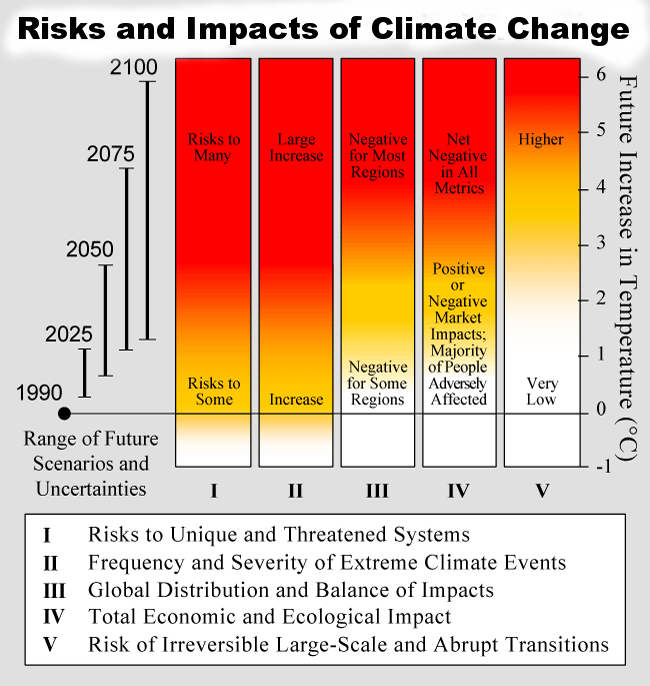
\includegraphics[width=0.6\textwidth]{img/Risks_and_Impacts_of_Global_Warming.png}
	\caption{'Burning embers' diagram~\cite{IPCC-workinggroup-01}}
	\label{fig:burning_embers}
\end{figure}

\subsection{The Kyoto Protocol}

Having recognised that developed countries are primarily responsible for the high levels of greenhouse gases in the atmosphere (due to the last 150 years of industrial development), the \textsc{unfccc} formed the Kyoto Protocol to not only encourage countries to reduce emissions, but to commit to it.~\cite{UNFCCC-kyoto-summary}

The initial agreement was signed on the 11th December 1997 during the 3rd annual \textsc{unfccc} conference and then came into force on the 16th February 2005. The Protocol sets mandatory targets on greenhouse-gas emissions for the world’s leading economies ``with a view to reducing their overall emissions of such gases by at least 5 percent below existing 1990 level in the commitment period 2008 to 2012.''~\cite{UNFCCC-98-p1}. Future targets are expected to be drawn up for ``commitment periods'' after 2012.~\cite{UNFCCC-98-p4}

As of September 2011, 191 countries have ratified the treaty with the United States remaining as the only signatory not to have ratified the protocol. However, certain United Nation member states such as Afghanistan, Andorra and South Sudan never signed the agreement and Canada left in December 2011.

The aim of the Kyoto Protocol is to contain emissions of anthropogenic \textsc{ghg}s in a way that reflects underlying national differences in emissions, wealth, and capacity for reduction; this concept is known as “common but differentiated responsibilities.”~\cite{Grubb-04}\cite{UNFCCC-92} It was recognised that much of the existing \CO emissions were due to developed countries, and that the needs of developing countries would need to be taken into account when calculating emission targets. It was agreed that the per capita emissions of developing countries was still relatively low, and that these participants would be allowed to grow to meet their socio-economic needs.

Participants in the Kyoto Protocol were classified into three groups, according to their responsibilities:~\cite{UNFCCC-92}

\begin{description}
	\item[Annex I] \hfill \\
	Industrialised countries and economies in transition. These countries have committed to reduce their emissions levels of greenhouse gases to targets that are set according to their 1990 emissions.
	
	\item[Annex II] \hfill \\
	Developed countries. Annex II countries are a subset of Annex I countries, and are encouraged to invest in developing countries.

	\item[Non-Annex I] \hfill \\
	Developing countries which are not required to reduce emission levels unless developed countries have supplied funding and technology through outsourcing. This serves three purposes
	\begin{itemize}
		\item There are no restrictions on the country’s development (as emissions are strongly linked to industrial capacity)
		\item Ability to sell emissions credits to those nations having difficulty meeting theirs.
		\item Encourages investment from Annex I countries for low-carbon technology.
	\end{itemize}
\end{description}

The Protocol structures rolling emission reduction commitment periods, with the first scheduled to end in 2012.

\subsubsection{2012 Targets}

Parties partaking in the Kyoto Protocol commit themselves to reducing four \textsc{ghg}s (carbon dioxide, methane, nitrous oxide, sulphur hexafluoride) and two other groups of gases (hydrofluorocarbons, perfluorocarbons). These are considered \CO equivalents when  calculating emission reduction.

With the understanding that only Annex I countries have targets that they must commit to, the aim is to reduce global \CO emissions to at least 5\% below the base year by the end of the first commitment period. Through negotiation, the base year decided on was 1990, due to the lack of accurate data for years prior to this. Participants would need to agree to their individual targets in line with the global target, the results of which can be seen in Table X. It should be noted that the \textsc{eu}-15 opted for a ‘burden-sharing agreement’ whereby the \textsc{eu} set a target of -8\%, and assigned individual targets to its member states.

[TABLE]

Countries can meet their targets by reducing their greenhouse gas output, or by offsetting their output by using the Flexible Mechanisms outlined in the Protocol. Even if Annex I countries meet their targets for the first period, future reductions will be required if the overall goal of \textsc{ghg} stabilisation is to become a reality.

\subsubsection{Flexible Mechanisms}

While participant countries must meet their emission targets primarily through domestic carbon reduction methods, Flexible Mechanisms were also put in place to make targets more attainable and affordable. These market based mechanisms help stimulate sustainable development through technology transfer, help countries with Kyoto commitments to meet their targets in a cost-effective way, and encourage the private sector and developing countries to contribute to emissions reduction. The three mechanisms defined in the Protocol are:

\begin{description}
	\item[Emissions Trading] \hfill \\
	Member states can trade a newly created commodity representing the surplus created if their emissions are below their assigned target.
	
	\item[Clean Development Mechanisms] \hfill \\
	Annex I \& II countries can invest in sustainable, greenhouse gas reduction projects in Non-Annex countries in exchange for “Certified Emission Reductions” \textsc{cer}).~\cite{UNFCCC-05}

	\item[Joint Implementation] \hfill \\
	Annex I countries can invest in sustainable greenhouse gas reduction projects in other Annex I countries as an alternative to national reduction.
\end{description}

\paragraph{International Emissions Trading}

With international markets already trading in commodities, Article 17 of the Protocol allows for countries to sell their excess “Assigned Amount Units” (\textsc{aau}s) to countries struggling to meet their target. This ability for countries to sell their excess capacity saw the birth of the “carbon market”.

Some Annex I countries, categorised as Economies In Transition (\textsc{eit}), have a large surplus of \textsc{aau}s, which can be sold on the carbon market. One example is Russia: having closed many cold-war-era industries since its 1990 base year, Russia was given more ‘headroom’ for growth when its carbon target was set. Despite the abundance of \textsc{aau}s in the market, to stop countries “overselling” units and becoming unable to meet their own targets, participants must keep a reserve of \textsc{aau}s (known as a “commitment period reserve”) which cannot fall below 90\% of its assigned amount.
European Union Emission Trading System

The European Union Emission Trading System (\textsc{eu ets}) allows for trading between participants in the EU and between industry operators in the \textsc{eu}. Governments of \textsc{eu} states agree on national emissions caps, and then allocate allowances to their industrial operators. Operators may privately move allowances between themselves, privately match buyers and sellers, or trade on the carbon exchange. It was found that other than trading has occurred in the global context of the Kyoto Protocol.~\cite{Grubb-09}

\paragraph{Clean Development Mechanisms}

Article 12 of the Protocol allows for Clean Development Mechanisms (\textsc{cdm}), whereby Annex I countries may invest in emission-reducing projects in developing countries. In exchange, projects earn saleable Certified Emission Reduction (\textsc{cer}) credits, which the investor may use to meet their target. Article 12 of the Protocol describes its objectives:

\begin{itemize}
	\item Assist Annex I parties to develop sustainable emission-reduction projects in Non-Annex countries (in line with the primary \textsc{unfccc} goal)
	\item Assist Annex I parties to meet their emission targets
\end{itemize}

Figure~\ref{fig:cdm_map} shows a map of CDM projects worldwide.

\begin{figure}[h!]
	\centering
	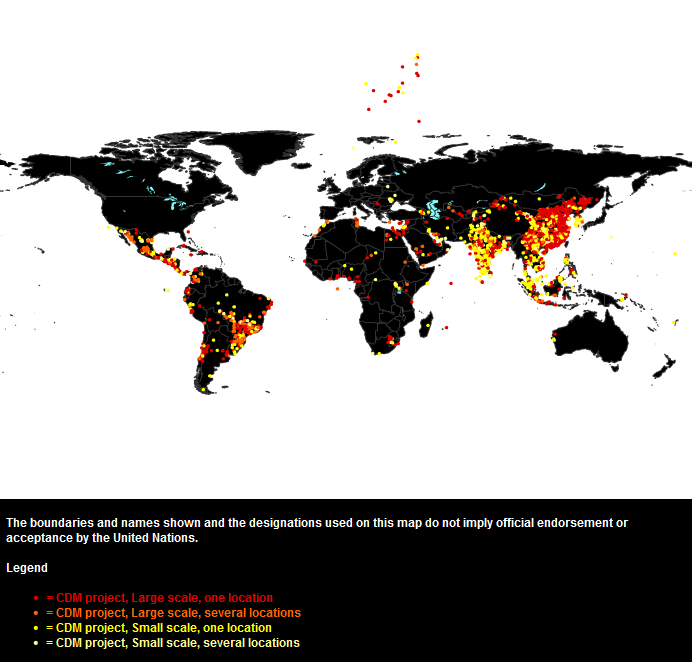
\includegraphics[width=0.8\textwidth]{img/CDM_Map.png}
	\caption{Map of \textsc{cdm} projects worldwide~\cite{UNFCCC-CDM-map}}
	\label{fig:cdm_map}
\end{figure}

Industrialised countries wishing to take part in \textsc{cdm} need to get assurance from the project host that it will contribute to sustainable development. The applicant must also prove that the project would not have happened regardless of their support, and must project future emissions had the project not gone forward (which are validated). This ensured there are no ‘free riders’, and that the applicant is awarded the correct amount of units for their contribution to the project.

\paragraph{Joint Implementation}

Article 6 defines the Joint Implementation (\textsc{ji}) mechanism, which allows countries to invest in carbon-reduction projects in other Annex I countries as an alternative to national emission reduction. In exchange for the investment, the investor will be awarded an Emission Reduction Unit (\textsc{eru}), which is to be taken from the investee’s \textsc{aau} pool. This requirement ensures that the total amount of units shared between Annex I countries does not change during a commitment period.

JI may be advantageous where carbon reduction is cheaper to implement in another Annex I country rather than nationally (an example might involve replacing dirty power plants with cleaner energy producers). To date, \textsc{ji} has not been very popular, with only 22 projects having been registered prior to 2008.

\subsubsection{Reporting, Monitoring and Sanctioning}

Each participant must designate an authority to create and manage its \textsc{ghg} inventory. While not specifically required, many non-annex countries have also set up national bodies to manage their Kyoto obligations (primarily \textsc{cdm}s).

Kyoto requires that:~\cite{UNFCCC-Kyoto-guidelines}

\begin{itemize}
	\item Annex I countries must have in place a national system to estimate \textsc{ghg} emissions (natural and anthropogenic), and any \CO that has been removed through sinks
	\item Annex I countries must report their greenhouse inventories annually, and provide regular communication detailing supplementary information to demonstrate compliance.
	\item Expert review teams periodically review greenhouse inventories and any national communications (This must be conducted at least once every 5 years)
\end{itemize}

It is understood that the effectiveness of the Kyoto Protocol depends on the participants following the Protocol’s rules and regulations with respect to their commitments the accuracy and reliability of the reports. Keeping in line with the core aim of the Kyoto Protocol (that is, an alternative to a carbon tax) financial sanctions were avoided, instead opting for the setting of harsher emissions targets.

Part of monitoring involves an expert review of reports submitted by participants. Reviewers may mark reports as “question of implementation” where there is an unresolved problem regarding implementation, may suggest “adjustment” where inventory is incomplete, and may suggest “correction” where there are clear inconsistencies (suggesting ‘cheating’). “Correction” is analogous to an inventory adjustment.~\cite{UNFCCC-reporting-review}

There are also sanctions for parties not meeting the emissions target they committed to. If the enforcement branch determines that Annex I countries do not comply with their emissions limitations, that country is required to make up the difference in future commitment periods plus an additional 30\%. That country will also be suspended from emissions trading.~\cite{UNFCCC-compliance}

\subsubsection{Problems}

Opinions on the effectiveness of the Kyoto Protocol vary significantly; while some consider it a move in the right direction for the stabilisation of \textsc{ghg}s, others believe the Protocol is inherently unfair, and ineffective.

Indeed some problems of fairness were raised early in the negotiation stages of the Protocol. During the negotiations for the setting of the base year, 1990 was chosen as reliable data prior to this date was unavailable. This base year was also highly favoured by the \textsc{uk}, Germany and Russia as their respective \CO levels were high in 1990. Following 1990, \textsc{uk} emissions dropped as the energy sector moved away from coal power, toward cleaner gas power stations. Germany’s \CO emissions also decreased following 1990 when East Germany and West Germany were reunited, resulting in a decrease in dirty industry in East German territories. There was much disagreement as Japan wished to use 1995 as the base year, while former Soviet block countries wanted to use emission rates from before their industrial collapse at the end of the cold war.

There were also disagreements over the size of the emission cuts, with the \textsc{eu} supporting cuts in the range of 10-15\%, while the US wanted a more conservative cut of between 0-5\%. The level of cutbacks wanted varied from country to country, with the only common theme being that the proposals suited the interests of the country making the proposal.~\cite{Grubb-economics}

There was also concern regarding the implementation of emissions trading. The \textsc{eu} and Japan wanted to ensure that emission trading was free and transparent, and wanted to prevent the \textsc{us} from using its political pressure to gain preference when trading with Russia. This concern was echoed in developing countries, where they believed the \textsc{us} would use flexibility mechanisms to its own advantage, over the interests of less able countries that needed support.

With Russia having an abundance of \textsc{aau}s, there was concern that it would have a monopoly on the carbon trading market, and would be able to adversely affect the price of carbon. Russia could withhold \textsc{aau}s to inflate the price for units, and inflate its profits. While possible, the situation was also difficult for Russia, since it has both an excess of \textsc{aau}s, and was one of the largest oil producers. Selling \textsc{aau}s would encourage the purchasing of oil, while withholding \textsc{aau}s would increase their value, but might adversely affect the price of fossil fuels.

\paragraph{The effect of Non-Annex countries}

Following successful negotiation and signing of the Protocol, concern was raised regarding the lack of limitations on the \textsc{ghg} emissions of developing countries. Indeed the \textsc{USA} did not ratify the Protocol, stating that "it exempts 80\% of the world, including major population centers such as China and India, from compliance, and would cause serious harm to the US economy".~\cite{Hague-to-marrakech} Statistics from the International Energy Agency (\textsc{iea}) show by 2011, emissions from Non-Annex I countries had exceeded those from Annex I countries.~\cite{CO2-fuel-highlights} Only 3 countries from the top 10 table of carbon emitters are currently an Annex I participants.

\subsection{Modeling the Kyoto Protocol as a Common Pool Resource}

\subsubsection{Common Pool Resource}

\subsubsection{Case Study}

\paragraph{Commercial fishing}

\paragraph{Ozone Layer \& \textsc{cfc}s}

\paragraph{Analysis}

\subsubsection{Mapping \textsc{cpr} to Kyoto}

\subsection{Multi-Agent Systems}

\subsubsection{Definition}

\subsubsection{Structure of an Agent}

\subsubsection{Services and Protocols}

\subsection{Presage 2}

\section{Defining our model}

\subsection{Time}

\subsection{Energy Output}

\subsection{Money}

\subsection{The Kyoto Protocol}

\subsection{Participants \& Actions}

\subsubsection{Domestic carbon reduction measures}

\subsubsection{Flexibility Mechanisms}

\subsection{Flowcharts}

\section{Implementation}

\subsection{Agents}

\subsubsection{Participants}

\paragraph{Annex I (Sustain)}

\subparagraph{Strategy}

\paragraph{Annex I (Reduce)}

\subparagraph{Strategy}

\paragraph{Non-Annex I}

\subparagraph{Unites States}

\subparagraph{Canada}

\subparagraph{Participant actions}

\paragraph{Carbon handlers}

\subparagraph{Carbon reduction}

\subparagraph{Reduction cost estimate}

\subparagraph{Carbon Absorption}

\subparagraph{Absorption cost estimation}

\paragraph{Energy handlers}

\paragraph{Carbon reporting}

\paragraph{Joining \& Leaving Kyoto}

\subsection{Protocols}

\subsubsection{Trade Protocol}

\paragraph{Functionality}

\paragraph{Reverting}

\paragraph{Trade Protocol state machine}

\paragraph{Initiator \textsc{fsm}}

\paragraph{Responder \textsc{fsm}}

\subsubsection{Time Service}

The time service is an environment service, extending Presage2’s existing environment interaction classes and development framework. It allows for coordination of time-based events and synchronises various features within our Kyoto Protocol simulation. Although Presage2 does have existing objects (SimTime) which can be used to attain simulation time, this is an absolute value in discrete logical time since the beginning of the simulation. It therefore does not take into consideration the variety of chronological distinctions the Kyoto Protocol requires, such as subdivisions into years and sessions.

It was initially decided to use a global service. It would perform most of the logic integral to coordinating time-driven activities, and would be layered on top of Presage2’s integrated SimTime object. However, it is necessary for agents to be able to query for information regarding the current year and session in order to make important strategic and behavioral decisions. Presage2 enforces that agents (participants) are unable to communicate directly with global services. While agents can act on the environment and affect services, performing the reverse is somewhat more complex.

At this stage, it would seem a participant time service would be more appropriate, since participant services can communicate directly with agents. However, another key functionality of the time service is the publishing of new events, both for the end of years and sessions, which trigger key monitoring, sanctioning, reporting, and architectural actions essential to the managed nature of the Kyoto Protocol. Unfortunately, implementation is not in place within Presage2 for participant services to generate (or interact with) the EventBus class, the object essential to publishing or receiving events.

With these restrictions in mind, the time service was subdivided into two separate services.   The participant service communicates with agents and relays information regarding the current year and session, among other minor time-related information gathering tasks. The global service is the backbone of the time service, generating new year and session events for the monitoring and targeting services to hook onto. It also carries out calculations to derive the current year and session from the discrete simulation time and communicates this information to the participant service.

Both classes extend from Presage2’s predefined EnvironmentService class, and use Google’s Guice injection systems for initialization and, in the global service’s case, to register with the EventBus.

\subsubsection{Monitor}

The monitor’s purpose is to regularly check whether countries are meeting their targets and randomly check for false carbon emission reports. If either case is true, a scaling sanction is applied to the country.

We were initially unsure whether the monitor should be an independent agent or an environment service. We settled on making it a service, so that it could listen to an event that would trigger the monitoring as agent are unable to do so.

When countries are initialised they subscribe to the monitor either as Annex I or Non Annex I. Although only Annex I countries are monitored, the Non-Annex I countries list was required to fix an issue with events at the end of a year happening in the right order. Indeed, countries were calling for their targets for the next year to be updated before the monitor could compare the results for the previous year against its previous targets. This was fixed by updating targets after the monitoring function in the Monitor service.

Every year the monitor charges the Annex I countries a tax, which is used to perform the monitoring action on randomly selected countries. If the monitor runs out of money, it cannot monitor and countries are free to behave without fear of sanction (although this information is hidden).

\subsubsection{Carbon Target}

\subsubsection{Market}

\subsection{Game Balancing}

% Got bored writing section titles here, just follow the standard set above%

\subsection{Kyoto \textsc{ui}}

\subsubsection{Overview}

The Kyoto \textsc{ui} is a web interface designed for instantiating and editing Presage 2 simulations. Web technologies used include an Apache web server, \textsc{php}, \textsc{html} and Javascript. Combined with a few additional libraries, these technologies provide the functionality required to display rich pages which allow for good visual representation and easy editing of data.

\subsubsection{Database Implementation}

The mongo database is interfaced using an \textsc{odm} (Object Document Mapper) library called mongorecord. This wraps interfaces for querying and writing the collections in the database with \textsc{php} classes which can be instantiated and used throughout the project.

\subsubsection{Simulation Initialisation Data Import and Export}

In order for any simulation to have a starting point, data must be imported containing information such as how long the simulation should run for and the data is required to set up each of the agents. Presage 2 has a command line interface which can be used to create simulations in the database and add parameters to them. The structure of these simulations in the database was used as a framework to import \textsc{csv} files of data to create simulations in the same format as generated by the Presage 2 \textsc{cli}.

\subsubsection{\textsc{csv} Import and Export Functionality}

To get data in and out of the system \textsc{csv} (Comma Separated Value) files are used. This is a convenient method of transferring data as the \textsc{csv} file can be opened and edited in spreadsheet software such as Microsoft Excel. Data collected on countries of the world is inserted into the simulations, as are parameters from ‘default’ \textsc{csv} files. Once these are in the database, the \textsc{ui} can copy and edit them. Simulations can then be exported as a backup or to transfer them to another database. This functionality underpins the whole simulation by providing an easy way to get a huge amount of data in and out of the system quickly, easily and reliably.

\subsubsection{Simulation Editor \textsc{ui}}

Once data has been imported from the \textsc{csv} file it may be necessary to make new simulations by changing parameters etc. This is one of the main tasks of the web \textsc{ui}, to make this editing visually comprehensive and easier than manually editing the \textsc{csv} file or the database entry.

\subsubsection{Agent (Country) Data}

Most agents in the simulation are countries and in order for the simulation to be as realistic as possible these are modelled on real countries with parameters describing land mass etc. stored in the database. It is useful to edit some of these parameters such as the percentage of land mass available for green development to investigate what happens in a simulation given agents with different parameters. In the \textsc{ui} there is a page specifically for editing countries which displays a clickable map of the world with a dropdown menu for country selection. This way all countries within a single simulation can be displayed as a bunch of editable parameters.

% UI IMAGE

The simulation overview page displays a world map using colour to indicate the values of a selected parameter for each country (default is arable land area percentage). There is a drop down menu (called Map View) which allows changing of the parameters displayed on the map. Below this is a table displaying a detailed output of all the simulation data from the database. This page also links to the \textsc{csv} export feature, copy feature, edit simulation page and a dropdown is present to allow editing of all the countries within the simulation.

\subsubsection{Simulation Results}

\bibliography{references}{}
\bibliographystyle{unsrt}

\end{document}
